%=======================================================================
%  ICISER 2026 / AIS SIGED -- SHORT PAPER.  Double-blind.
%
%  CFP: 2500-4500 words body, abstract <=150, must state motivation,
%  research design and expected contributions.  Research-in-progress
%  and early findings are explicitly welcome.
%
%  STATUS.  Dataset construction, splitting, auditing, the corpus finding,
%  and both full 15-fold sweeps (deberta-v3-small and roberta-base, seed
%  42) are measured and reported.  Every figure and number comes from
%  notebooks/GRADE_figures.ipynb.  A multi-seed sweep remains open.
%=======================================================================
\documentclass[11pt,a4paper]{article}

\usepackage[margin=1in]{geometry}
\usepackage{times}
\usepackage{amsmath,amssymb}
\usepackage{booktabs}
\usepackage{graphicx}
\usepackage{multirow}
\usepackage{url}
\usepackage{xcolor}
\usepackage[hidelinks]{hyperref}
\usepackage{titlesec}
\titleformat{\section}{\normalfont\large\bfseries}{\thesection.}{0.5em}{}
\titleformat{\subsection}{\normalfont\normalsize\bfseries}{\thesubsection.}{0.5em}{}

% 12 floats in a short paper: give LaTeX room before they spill
\renewcommand{\topfraction}{0.95}
\renewcommand{\bottomfraction}{0.85}
\renewcommand{\textfraction}{0.05}


\renewcommand{\floatpagefraction}{0.6}
\setcounter{topnumber}{3}
\setcounter{bottomnumber}{2}
\setcounter{totalnumber}{4}

\title{\textbf{GRADE: Do AI-Text Detectors Survive the Next\\
Assignment, and Who Pays When They Fail?}}

% DOUBLE-BLIND: \author{} stays empty for submission.
% For the camera-ready, delete this comment block and uncomment the
% \author macro below.
%
% \author{
% Muhammad Yousaf Rehman\\
% SPECS, University of Hertfordshire\\
% Hatfield, United Kingdom
% \and
% Muhammad Islam\\
% College of Science and Engineering, James Cook University\\
% Cairns, QLD, Australia
% }
\author{}
\date{}

\begin{document}
\maketitle
\vspace{-2.5em}

%----------------------------------------------------------------- abstract
\begin{abstract}
\noindent
Generative AI has unsettled written assessment, and universities now screen
student essays with AI-text detectors reporting accuracies above 99\%,
usually cross-validated on the very corpus they are scored against. We introduce GRADE (Generalization
Robustness Assessment for Detectors in Education), a
leave-one-assignment-out evaluation over 44{,}861 student essays across 15
assignments that attributes every false accusation to the student who
wrote it. Against a word-frequency baseline fitted on every
fold, accuracy on an unseen assignment stays high (93--100\%), yet the
baseline matches or beats \texttt{deberta-v3-small} on 9 of 15 folds and
\texttt{roberta-base} on 8: high accuracy is not evidence of detecting
authorship. Both exceed 99.6\% ROC-AUC everywhere, locating the failure in
the decision threshold, not the representation.
False accusations also fall 5.6 times as often on the most-highly-graded
students as on the least, traced to formal style rather than grade. We release the merged, deduplicated corpus with
assignment labels and named generators.
\end{abstract}

\begin{center}
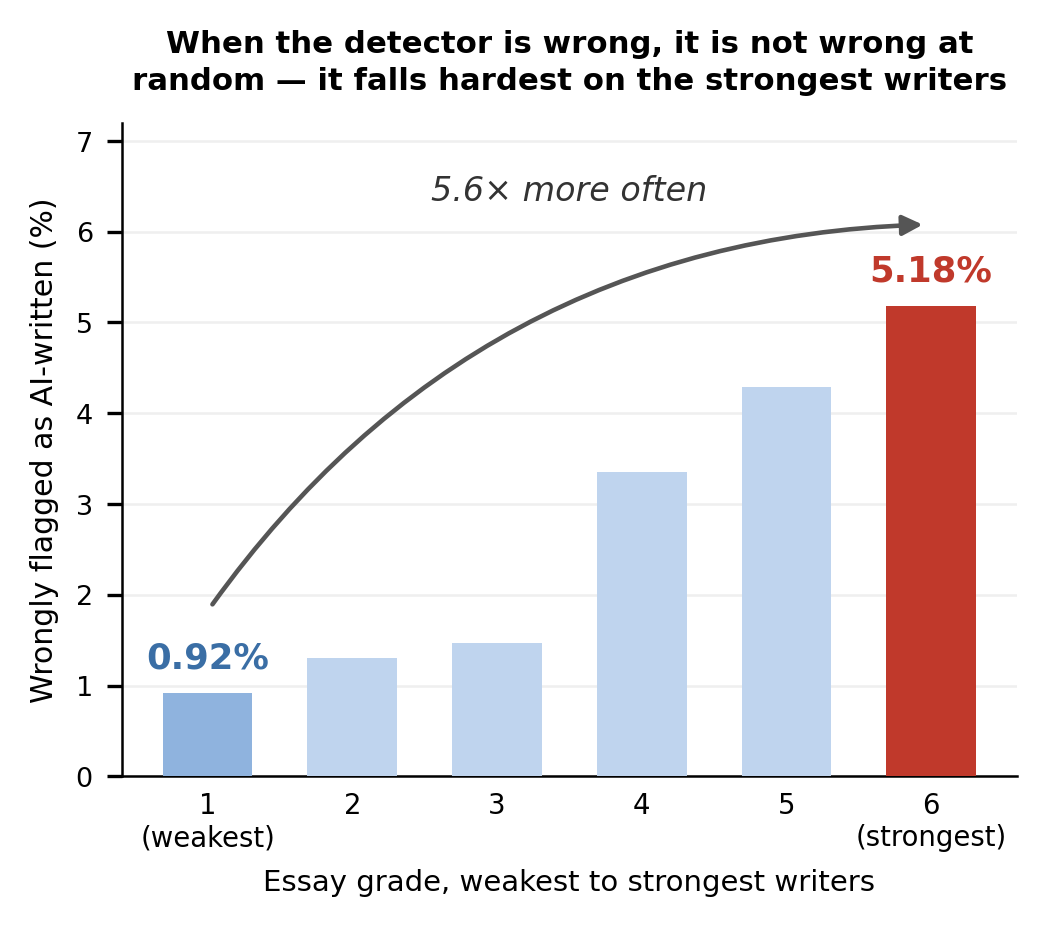
\includegraphics[width=0.48\textwidth]{Assets/teaser_fairness.png}\\[2pt]
{\small\itshape When the detector is wrong it is not wrong at random: false
accusations on authentic student work rise 5.6-fold from the weakest to the
most-highly-graded writers (Table~\ref{tab:fairness}).}
\end{center}
\vspace{-0.8em}

\vspace{0.5em}
\noindent\textbf{Keywords:} academic integrity, assessment, generative
AI, AI-text detection, algorithmic fairness, evaluation methodology.

%=======================================================================
\section{Introduction}
%=======================================================================

A student can now produce a competent essay without doing the thinking the
essay was set to evidence. Generative language models have made this easy
enough that institutions are under pressure to respond, and one response
is technical: adopt a detector, run submissions through it, and treat the
output as evidence in academic-integrity processes.

That response is justified by numbers. Recent work reports Macro F1 scores
of 99.78\% and 98.10\% for fine-tuned detectors, rising to 100.00\% on one
corpus \cite{qorich2025}. Commercial detectors report comparably high
figures. Read at face value, the problem looks solved.

It is not solved. Those figures are measured on the corpus the detector was
built from. The essays it is scored against answer the same assignments,
come from the same cohort, and were generated by the same models as the
essays it learned from. Choosing a stronger architecture does not close
this gap, because the number being compared across architectures is
itself measured the same way: on assignments the detector has already
seen scored. A programme director needs two other things no such number
speaks to: what happens with next semester's assignment, which by
definition no detector has been scored against yet, and what happens to
the students the tool gets wrong.

Adopting a detector is an information-systems decision. It places an
automated classifier inside a consequential process about students, with
sanctions attached to its output. IS scholarship holds that a system's
success is measured by its fit to the task and the outcomes it produces in
actual use, not by a property intrinsic to the system alone
\cite{delone2003}. A review of algorithmic decision tools already deployed
across higher education finds the reverse practice: proposals are assessed
on model performance and rarely on the governance, interpretability or
downstream consequences of deploying them \cite{mcconvey2023}. Detection
tools are being adopted the same way. This paper therefore concerns an
intelligent system deployed \emph{by} educators to govern assessment,
rather than the generative systems students use.

We ask two questions.

\textbf{RQ1.} If a detector is trained on a set of assignments and then
meets an assignment absent from training, how much of its reported
performance survives?

\textbf{RQ2.} When it is wrong about authentic student work, which students
absorb the error?

RQ1 isolates the one shift a programme cannot avoid. Every term brings a
new assignment. RQ2 asks what an aggregate accuracy conceals, because a
false positive is not a statistical event. It is an accusation against a
named student. Our contributions are:

\begin{itemize}
\item We introduce a leave-one-assignment-out protocol that measures
transfer to a genuinely unseen assignment, rather than to a held-out
sample of the same assignments a detector trained on.
\item We fit a word-frequency control on every fold and show it is
sufficient, on a majority of folds, to match a fine-tuned transformer,
so the accuracy a detector reports is not by itself evidence of
detecting authorship. Two encoders reproduce this, and their ROC-AUC
places the loss on the threshold, not the representation.
\item We join detector verdicts to teacher-assigned grades and writer
characteristics for the same essays, and show the false-positive rate
rises with grade rather than falling on it, then test and support a
formality mechanism for why.
\end{itemize}

%=======================================================================
\section{Literature Review}
%=======================================================================

Detecting generated text is usually posed as supervised binary
classification. A pretrained encoder is fine-tuned on a corpus pairing
human-written documents with generated ones, and the resulting classifier
is scored on held-out items from that same corpus. The encoder supplies
the representation and the corpus supplies the notion of what generated
text looks like, so both the reported accuracy and its meaning depend on
how that corpus was assembled and divided. Qorich and El Ouazzani are
representative of the strongest current results in this line: they
fine-tune GPT-2, RoBERTa and BART across five corpora and report the
figures quoted above \cite{qorich2025}, measuring generalization by
five-fold cross-validation on each target corpus in turn.

The difficulty is what that protocol can establish. Cross-validation
trains on four fifths of the corpus it evaluates, so the essays a detector
is scored against answer the same prompts, come from the same cohort and
were produced by the same generators as the essays it learned from. A
detector that had memorised the vocabulary of those particular prompts,
and learned nothing transferable to a corpus assembled elsewhere, would
still score well under it. The same design constrains what can be said
about who a detector gets wrong: a group difference under 2\% is reported
for essays that carry no demographic field \cite{qorich2025}, so the claim
has no grouping variable behind it. Neither limitation is peculiar to that
study. Both follow from an evaluation protocol the field has largely
settled on, and together they set the two questions this paper asks.

Work situated in education reaches conclusions that are difficult to
reconcile with accuracies above 99\%. Weber-Wulff et al. evaluate fourteen
detection tools, including commercial ones marketed to universities, and
conclude that none is reliable enough for academic-integrity decisions,
with accuracy degrading further once text is lightly obfuscated
\cite{weberwulff2023}. Sadasivan et al. argue the problem may be harder
still, giving theoretical grounds and empirical evasions suggesting
reliable detection may not be achievable as generated and human text grow
closer in distribution \cite{sadasivan2023}. Liang et al. matter most to
the question of who absorbs the error: they show detectors flag writing by
non-native English speakers as generated far more often than writing by
native speakers, and attribute this to lower lexical variety being read as
a machine signature \cite{liang2023}. That finding is bounded by its
design, because the non-native and native writing come from different
sources, so writer group and corpus vary together and the effect cannot be
separated from whatever else distinguishes the two collections. Whether
the same gap appears between writers inside one cohort, answering the same
assignment and marked by the same raters, is open --- and that is the form
a university would actually meet.

Robustness under distribution shift is by now an established concern, and
the benchmarks built to measure it are explicit about which shift they
vary. RAID spans eleven generators, eight domains and eleven adversarial
attacks, and finds that detectors, commercial ones included, degrade
sharply outside the conditions they were tuned on \cite{raid2024}. MAGE
reports substantial degradation when the generator at test time was not
seen in training \cite{mage2024}, and paraphrasing is a well-documented
evasion strategy against detectors that were never shown paraphrased text
\cite{krishna2023}. Between them these studies vary the generator, the
genre and the provenance of the text. None of those is what changes inside
a running course: the cohort, the marking scheme and the tools available
to students stay largely fixed from one term to the next, while the
assignment itself is replaced. We are not aware of a study that isolates
that shift.

Two gaps follow from this literature. The shift a teaching programme
actually meets, a new assignment set to the same cohort, has not been
measured; and no study reports which students absorb a detector's false
accusations when it is wrong. GRADE addresses both.

%=======================================================================
\section{Dataset Collection}
%=======================================================================

Answering RQ1 and RQ2 requires a corpus of student essays large enough to
support 15 held-out folds, labelled with the assignment each essay answers,
and joinable to real writer information. No single public release offers
all three, so the corpus used here is built from two collections of the
same student writing, merged and deduplicated, with a third collection
supplying the writer information. Table~\ref{tab:data} summarises the
result.

\subsection{Student essays}

Both collections draw their student essays from the PERSUADE corpus:
25{,}996 argumentative essays written by United States students in grades 6
to 12 across 15 assignments \cite{crossley2024}. The first is the corpus
released for the LLM-Detect competition organised by Vanderbilt University
and The Learning Agency Lab \cite{king2023}. The second is a
community-assembled corpus for the same task, pairing the PERSUADE essays
with generated essays from 16 named models including Llama-2, Mistral,
Claude, PaLM and Falcon \cite{daigt2024}.

Only the community corpus records which assignment each essay answers, and
65\% of the competition corpus is already contained within it, so every
labelled essay in the study comes from the community corpus:
\textbf{44{,}861 essays across 15 assignments}. We match the two on
normalised text rather than stacking them, because stacking would place the
same essay in the corpus twice and let a later split put one copy in
training and the other in test, which is the arrangement this paper
criticises. Two essays carried conflicting labels across the sources and
were discarded, and 9{,}481 competition essays that no assignment label
covers are excluded rather than assigned by inference.

\subsection{Writer information}

PERSUADE records, for each essay, the holistic grade awarded by human
raters on a 1 to 6 scale, the word count, the school year, whether English
is an additional language for the writer, and indicators of economic
disadvantage and disability \cite{crossley2024}. Grades are present for
100\% of essays and English-language status for 95\%. Matched on exact
text, PERSUADE covers \textbf{25{,}995 of the 27{,}367 student essays} in
our corpus, or 95\%.

PERSUADE contains no generated text. It is therefore never trained on. It
is a reference layer applied to the detectors' verdicts, and it is what
makes RQ2 answerable.

\begin{table}[tb]
\centering
\small
\caption{The corpus. Two collections of the same student writing are merged
and deduplicated; a third supplies grades and writer characteristics and is
never trained on.}
\label{tab:data}
\begin{tabular}{@{}p{2.6cm}p{2.0cm}rr@{}}
\toprule
\textbf{Collection} & \textbf{Role} & \textbf{Items} & \textbf{Student:AI} \\
\midrule
LLM-Detect \cite{king2023} \newline
{\footnotesize no assignment label} &
merged & 29{,}145 & 17{,}508 : 11{,}637 \\
\addlinespace
Community corpus \cite{daigt2024} \newline
{\footnotesize 15 assignments, 16 generators} &
merged & 44{,}868 & 27{,}371 : 17{,}497 \\
\addlinespace
\textbf{Merged, labelled} \newline
{\footnotesize deduplicated; used here} &
train / stop / mark & \textbf{44{,}861} & \textbf{27{,}367 : 17{,}494} \\
\addlinespace
PERSUADE 2.0 \cite{crossley2024} \newline
{\footnotesize grades, writer characteristics} &
reference only & 25{,}996 & 25{,}996 : 0 \\
\bottomrule
\end{tabular}
\end{table}

%=======================================================================
\section{Methodology}
%=======================================================================

The protocol has three parts: a detector fine-tuned the same way on every
fold, a leave-one-assignment-out split that rotates which assignment is
withheld, and an attribution step that joins the detector's verdicts back
to the writer who produced each essay. Figure~\ref{fig:arch} gives an
overview before each part is described in turn.

\begin{figure*}[tb]
\centering
% uncomment once the diagram is exported to Assets/:
\includegraphics[width=\textwidth]{Assets/grade_arch.pdf}
\caption{The GRADE protocol. Two corpora are merged and deduplicated into
44{,}861 student essays across 15 assignments. One assignment is held out
at a time: the detector is fine-tuned under one recipe on the remaining 14
and marked on the one withheld. Three properties are enforced rather than
assumed, and control comparisons that cannot recognise authorship are
fitted separately on every fold. Teacher-assigned grades and writer
characteristics are then joined to the verdicts, so each false accusation
is attributed to the student who wrote the essay.}
\label{fig:arch}
\end{figure*}

\subsection{Detectors}

We fine-tune two parameter-matched, architecturally distinct encoders
end-to-end for binary classification of student versus generated writing.
The first is \texttt{deberta-v3-small}, roughly 140M parameters, whose
disentangled attention decomposes the score between positions $i$ and $j$
into content-to-content, content-to-position and position-to-content
terms. The second is \texttt{roberta-base}, roughly 125M parameters,
comparably sized but architecturally simpler, computing a single
undecomposed attention over content and position jointly. Both truncate to
256 tokens and pass the contextual \texttt{[CLS]} representation to a
feed-forward head returning $P(\mathrm{student})$ and
$P(\mathrm{generated})$.

We run the full rotation twice, once per encoder, not to rank the two but
to establish whether what the rotation exposes is a property of detectors
or of one model. DeBERTa-v3 is the strongest standard encoder at this size
and RoBERTa the most widely deployed, so a failure to transfer is not
attributable to a weak choice of model. Encoders of this kind underlie the
commercial tools now marketed to universities.

Table~\ref{tab:recipe} gives the training configuration. It is identical
across both encoders and all 15 folds, and nothing in it is tuned per
assignment, so a difference between folds reflects the assignment rather
than the effort spent on it.

\begin{table}[tb]
\centering
\small
\caption{Training configuration, fixed before the first fold and identical
across both encoders, all 15 folds and the in-fold controls.}
\label{tab:recipe}
\begin{tabular}{@{}ll@{}}
\toprule
\textbf{Setting} & \textbf{Value} \\
\midrule
Conditions        & \texttt{deberta-v3-small}, \texttt{roberta-base} \\
Initialisation    & pretrained checkpoint, fresh head \\
Max token length  & 256 \\
Optimiser         & AdamW \\
Learning rate     & $2\times10^{-5}$ \\
Batch size        & 8 \\
Epochs            & 5 \\
Loss              & cross-entropy \\
Fine-tuning       & full, encoder and classifier \\
Checkpoint        & best on the stopping portion \\
Random seed       & 42 \\
Total runs        & 15 folds $\times$ 2 encoders $=$ 30 \\
\bottomrule
\end{tabular}
\end{table}

\subsection{The leave-one-assignment-out protocol}
\label{sec:protocol}

The intuition is familiar from masked language modelling, where tokens are
hidden and then recovered from the context around them. GRADE masks at a
different granularity and for the opposite purpose: the unit is an entire
assignment rather than scattered tokens, and recovering any of it from
training would be contamination rather than success. Formally the protocol
is grouped cross-validation with the assignment as the group, in the manner
of leave-one-subject-out designs in clinical machine learning.

Let $\mathcal{A}$ be the set of 15 assignments. For each held-out
assignment $a \in \mathcal{A}$ we define

\begin{align}
\mathrm{Train}(a) &= \mathcal{A} \setminus \{a\}, \\
\mathrm{Test}(a)  &= \{a\}.
\end{align}

The 14 assignments in $\mathrm{Train}(a)$ are divided 85\% to fit the
detector and 15\% to decide when to stop fitting it. The withheld
assignment contributes no essay to either portion and is opened once, at
the end. Every test decision therefore concerns an assignment absent from
training, and rotating $a$ over all 15 gives a complete picture rather than
a single sample, separating the difficulty of an assignment from the
difficulty of the task.

Cohort, marking scheme and generators are held fixed across folds; only the
assignment differs. That is the shift a programme meets when it sets new
coursework, and it is the one shift a programme cannot avoid.

The excluded essays matter here because any of them could belong to the
assignment being withheld. A topic classifier accurate to 97.4\% on known
assignments places 62\% of them with no confidence, indicating sources
beyond the 15 and confirming they cannot be assigned safely.

\subsection{What the split guarantees}

A split of this kind can leak in ways that would flatter the detector, and
this corpus is unusually exposed to one of them: it is merged from two
collections that overlap, so the same essay text arrives from more than one
source row. Left unhandled, that would let a detector score well by
recognising an essay it had already seen rather than by detecting
authorship. The folds themselves are defined on recorded assignment labels
rather than inferred ones, so the second obvious risk does not arise.

We therefore enforce three properties on every fold rather than assuming
them. No essay from the held-out assignment appears in training or in the
stopping portion, so the test assignment is genuinely unseen. No text
appears in more than one of the three portions, so a duplicated essay
cannot be memorised in training and recognised in test. And every portion
carries equal numbers of student-written and generated essays, which fixes
a guessing detector at 50\% and makes folds comparable to one another.

Each property is checked by an audit that raises and halts the study rather
than issuing a warning, so a violation cannot pass unnoticed into a
reported number. All 15 folds pass all three checks.

\subsection{Controls}

Accuracy alone cannot say whether a detector has learned anything about
authorship, because a method that plainly has not may reach the same
number. Alongside every detector we therefore fit two deliberately
unintelligent comparisons, each refitted on that fold's training portion so
that it meets the same held-out assignment under the same conditions as the
detector it is being compared with.

The first sees a single number per essay: its length. The second sees which
words appear and how often, with no sense of their order or meaning.
Neither has any notion of who wrote a text, so whatever they score is
reachable without recognising authorship. A detector must beat them before
its accuracy can be credited to anything about writing.

The two ask questions of different difficulty. Length asks whether the
detector does more than count characters, and is a low bar on this corpus
by construction: the median student essay is 2{,}131 characters against
1{,}974 generated, a ratio of 1.08 to 1. Word frequency asks the harder
question of whether it does more than count words, and it is refitted per
fold because that length balance does not hold on every assignment.

\subsection{Attributing the errors}

For RQ2 we take every authentic essay in a held-out assignment, join the
detector's verdict to what PERSUADE records about its writer, and report
the false-positive rate per group. Only authentic work enters this
analysis, because only authentic work can be falsely accused. The join is
on the essay identifier rather than on row order, so it does not depend on
the two sources being aligned.

A rate that varies by group is a correlation and not yet an explanation, so
we also test one mechanism, described with its result in
Section~\ref{sec:mechanism}. If that test comes back empty we report the group effect as
unexplained rather than reach for a cause.

%=======================================================================
\section{Evaluation}
%=======================================================================

Generated text is the positive class and student writing the negative
class. We report accuracy, recall and ROC-AUC in the tables, and both
error rates in the text where they carry the argument: the false-positive
rate is the share of genuine student essays wrongly flagged, the
false-negative rate the share of generated essays passed as authentic.
The false-positive rate carries most of the argument here, because a
false positive is an accusation against a named student.

Training is stochastic, so a difference between two folds could reflect the
assignment or the run. We therefore rest the argument on aggregates over
the 30 runs and on differences large enough to survive run-to-run
variation, and treat the ordering of adjacent folds as provisional.
Tables~\ref{tab:loto} to~\ref{tab:encoders} give the full results.

\subsection{RQ1: transfer}

The detector transfers. Accuracy ranges from 93.47\% (Exploring Venus) to
99.61\% (Car-free cities), a spread of 6.1 points, and it clears the
length-only control on every fold, by 13 to 50 points and 34.0 on average.
Read alone, this is the number a vendor would quote: an unseen assignment
costs a programme almost nothing.

Read against the word-frequency control, it is a different result. The
detector loses to that control on 9 of the 15 folds, by a mean of 0.76
points and by as much as 5.25 on Exploring Venus, its own worst fold. A
classifier with no notion of authorship, built from which words appear and
how often, matches or beats a fine-tuned transformer more often than not
under the exact shift this paper studies.

This is the answer to RQ1. Performance survives the shift almost
completely, but what survives is not shown to be detection of authorship
rather than of vocabulary. The margin that would demonstrate it is absent
on a majority of folds (Figure~\ref{fig:margins}).

\begin{figure}[tb]
\centering

\includegraphics[width=0.86\columnwidth]{Assets/rq1_margin_vs_control.pdf}
\caption{Accuracy minus the word-frequency control on each held-out
assignment, both encoders. Bars to the left of zero are assignments where a
method that cannot recognise authorship scored at least as well as the
fine-tuned detector.}
\label{fig:margins}
\end{figure}

\begin{table}[tb]
\centering
\small
\caption{Leave-one-assignment-out, all 15 folds, seed 42. Each row trains
on the other 14 assignments and marks only the one named. Generated text
is the positive class; all figures are percentages. Both controls are
fitted separately on each fold and cannot recognise authorship; positive
margins favour the detector.}
\label{tab:loto}
\begin{tabular}{@{}lrrrrr@{}}
\toprule
\textbf{Held-out assignment} & \textbf{Test $n$} &
\textbf{Acc.} & \textbf{Recall} & \textbf{vs.\ length} & \textbf{vs.\ TF-IDF} \\
\midrule
Distance learning                     & 4{,}314 & 98.79 & 98.70 & +22.4 & $-$0.65 \\
Car-free cities                       & 4{,}102 & 99.61 & 99.85 & +44.6 & +0.29 \\
Does the electoral college work?      & 3{,}440 & 99.48 & 99.94 & +44.5 & +0.52 \\
Seeking multiple opinions             & 3{,}104 & 96.01 & 99.16 & +24.1 & $-$2.19 \\
Mandatory extracurricular activities  & 2{,}812 & 98.36 & 99.43 & +24.1 & $-$0.64 \\
Summer projects                       & 1{,}902 & 97.79 & 99.26 & +13.1 & $-$1.37 \\
Facial action coding system           & 1{,}834 & 99.24 & 98.91 & +43.5 & +0.76 \\
Community service                     & 1{,}100 & 98.64 & 99.45 & +33.9 & +0.09 \\
``A Cowboy Who Rode the Waves''       & 1{,}046 & 96.46 & 99.81 & +33.9 & $-$3.16 \\
Grades for extracurricular activities &    980 & 99.18 & 99.18 & +32.2 & $-$0.41 \\
Cell phones at school                 &    926 & 99.46 & 99.57 & +37.4 & $-$0.11 \\
Phones and driving                    &    830 & 98.67 & 99.04 & +34.3 & +1.08 \\
Driverless cars                       &    728 & 99.59 & 99.73 & +49.6 & +0.69 \\
Exploring Venus                       &    628 & 93.47 & 100.00 & +40.6 & $-$5.25 \\
The Face on Mars                      &    620 & 96.94 & 96.45 & +31.1 & $-$1.13 \\
\midrule
\textbf{Mean over folds}              &        & 98.11 & 99.23 & +34.0 & $-$0.76 \\
\textbf{Worst fold}                   &        & 93.47 & 96.45 & +13.1 & $-$5.25 \\
\midrule
\emph{word-frequency control, mean}   &        & 98.88 & & & \\
\emph{length-only control, mean}      &        & 64.16 & & & \\
\bottomrule
\end{tabular}
\end{table}

\subsection{Not an artefact of one encoder}

Repeating all 15 folds with \texttt{roberta-base} leaves the aggregate
picture unchanged. The two encoders are indistinguishable on every summary
measure in Table~\ref{tab:encoders}, and RoBERTa loses to the
word-frequency control on 8 folds against DeBERTa's 9. Changing the encoder
does not recover the margin, so the finding belongs to the evaluation
rather than the model. Where they differ is more informative: each one's
worst assignment is close to the other's best, and their margins correlate
at $-0.15$ across the 15 folds, which is to say not at all. One detector's
weak assignment is no warning for another's.

Neither collapse is representational. ROC-AUC never falls below 99.68\% for
either encoder (Figure~\ref{fig:calibration}), so both rank essays
correctly on every assignment; on its worst fold RoBERTa still recovers only
80.17\% of generated essays at the default cut point. What fails is the
decision threshold, fitted where the assignment was seen and not travelling
with the ranking.

Re-scoring each fold at the cut point that maximises accuracy on it bounds
what better calibration could buy (Figure~\ref{fig:threshold}). The two
worst folds recover to 98.84\% and 97.61\%, and they need opposite
corrections, 0.025 against 0.985, so no single fixed threshold would have
served both. No detector can perform the correction anyway, because
choosing that cut point requires the labels for the assignment being
marked. The bound is the important part: given the threshold it could not
have known, each encoder still clears the word-frequency control on only 9
of the 15 folds, by 0.21 and 0.46 points on average. Calibration explains
where the accuracy went; it does not supply the evidence of detecting
authorship that the control was there to test for.

\begin{figure}[tb]
\centering

\includegraphics[width=0.62\columnwidth]{Assets/roc_auc_vs_accuracy.pdf}
\caption{Ranking survives the shift; the threshold does not. ROC-AUC stays
above 99.6\% on every fold for both encoders, while accuracy falls to
93.47\% for DeBERTa on Exploring Venus and 90.06\% for RoBERTa on the
electoral college.}
\label{fig:calibration}
\end{figure}

\begin{figure}[tb]
\centering

\includegraphics[width=0.58\columnwidth]{Assets/threshold_headroom.pdf}
\caption{Accuracy at the default cut point, with the shaded extension
showing what a threshold chosen on the held-out assignment itself would
recover. The correction is unavailable in use: it needs the labels the
detector is being asked to supply.}
\label{fig:threshold}
\end{figure}

\begin{table}[tb]
\centering
\small
\caption{Two encoders over the same 15 folds, seed 42, identical recipe.
$\Delta$ is accuracy minus the word-frequency control fitted on that fold.
Both encoders rank almost perfectly on every assignment; both lose accuracy
where the decision threshold does not transfer.}
\label{tab:encoders}
\begin{tabular}{@{}lrrrrrr@{}}
\toprule
& \multicolumn{2}{c}{\textbf{DeBERTa-v3}} & \multicolumn{2}{c}{\textbf{RoBERTa}}
& \multicolumn{2}{c}{\textbf{$\Delta$ vs control}} \\
\cmidrule(lr){2-3}\cmidrule(lr){4-5}\cmidrule(lr){6-7}
\textbf{Held-out assignment} & \textbf{Acc} & \textbf{AUC} & \textbf{Acc}
& \textbf{AUC} & \textbf{DeB} & \textbf{RoB} \\
\midrule
Distance learning            & 98.79 & 99.85 & 96.64 & 99.80 & $-$0.65 & $-$2.80 \\
Car-free cities              & 99.61 & 99.99 & 99.59 & 99.99 & +0.29 & +0.27 \\
Electoral college            & 99.48 & 100.00 & 90.06 & 99.85 & +0.53 & $-$8.89 \\
Seeking multiple opinions    & 96.01 & 99.68 & 98.16 & 99.97 & $-$2.19 & $-$0.04 \\
Mandatory extracurriculars   & 98.36 & 99.82 & 98.12 & 99.68 & $-$0.64 & $-$0.88 \\
Summer projects              & 97.79 & 99.81 & 97.21 & 99.77 & $-$1.37 & $-$1.95 \\
Facial action coding         & 99.24 & 99.97 & 99.84 & 99.99 & +0.77 & +1.37 \\
Community service            & 98.64 & 99.97 & 99.82 & 100.00 & +0.09 & +1.27 \\
A Cowboy Who Rode the Waves  & 96.46 & 99.96 & 98.47 & 99.97 & $-$3.16 & $-$1.15 \\
Grades for extracurriculars  & 99.18 & 99.94 & 99.08 & 99.99 & $-$0.41 & $-$0.51 \\
Cell phones at school        & 99.46 & 99.97 & 99.35 & 99.99 & $-$0.11 & $-$0.22 \\
Phones and driving           & 98.67 & 99.97 & 97.71 & 99.94 & +1.07 & +0.11 \\
Driverless cars              & 99.59 & 99.99 & 99.45 & 100.00 & +0.69 & +0.55 \\
Exploring Venus              & 93.47 & 99.98 & 99.84 & 100.00 & $-$5.26 & +1.11 \\
The Face on Mars             & 96.94 & 99.70 & 99.35 & 99.99 & $-$1.12 & +1.29 \\
\midrule
\textbf{Mean}                & 98.11 & 99.91 & 98.18 & 99.93 & $-$0.76 & $-$0.70 \\
\textbf{Folds above control} &       &       &       &       & 6/15 & 7/15 \\
\bottomrule
\end{tabular}
\end{table}

\subsection{RQ2: who absorbs the error}

The false-positive rate rises with grade at every step, from 0.92\% at
grade 1 to 5.18\% at grade 6, a 5.6-fold increase with no reversal across
the six bands. English-language status shows the same shape in the
opposite direction to prior work: writers for whom English is an
additional language are flagged at 0.63\%, against 2.87\% for other
writers, a 4.6-fold difference. Prior work finds non-native writers
over-flagged; here, inside one corpus with grade and rater held fixed,
they are under-flagged. The two results answer RQ2 the same way: the
detector's few mistakes are not spread evenly across students, and they
concentrate on writers whose English is judged the strongest by an
independent human rater, not the weakest. Table~\ref{tab:fairness} gives
both breakdowns and Figure~\ref{fig:fairness} plots them for both encoders,
which show the same gradient. The comparison with Liang et al. \cite{liang2023} is
cleaner in one respect: both writer groups here sit inside the same corpus
and are marked by the same raters, so group and corpus do not vary
together as in their design.

\begin{figure}[tb]
\centering

\includegraphics[width=0.92\columnwidth]{Assets/rq2_false_accusations.pdf}
\caption{False accusations on authentic student work, by holistic grade and
by English-language status, for both encoders. The gradient is a property
of the task rather than of one model.}
\label{fig:fairness}
\end{figure}

\begin{table}[tb]
\centering
\small
\caption{The false-positive rate on authentic student work, pooled over the
15 held-out folds. Every figure is an accusation against a student who did
their own work.}
\label{tab:fairness}
\begin{tabular}{@{}lrr@{}}
\toprule
\textbf{Writer group} & \textbf{Essays} & \textbf{False-positive rate} \\
\midrule
\multicolumn{3}{@{}l}{\emph{by holistic grade}} \\
\quad 1 (weakest)   & 434   & 0.92 \\
\quad 2             & 2{,}314 & 1.30 \\
\quad 3             & 3{,}805 & 1.47 \\
\quad 4             & 3{,}846 & 3.35 \\
\quad 5             & 2{,}166 & 4.29 \\
\quad 6 (strongest) & 637   & 5.18 \\
\midrule
\multicolumn{3}{@{}l}{\emph{by English-language status}} \\
\quad English an additional language     & 1{,}271  & 0.63 \\
\quad English not an additional language & 11{,}483 & 2.87 \\
\bottomrule
\end{tabular}
\end{table}

\subsection{Why formality drives it}
\label{sec:mechanism}

A rate that rises with grade is a correlation, not yet a mechanism, so we
test one directly rather than infer it from Table~\ref{tab:fairness} alone.
The mechanism we test is formality. Generated essays in this corpus carry
formal discourse markers at roughly four times the rate of student essays,
4.98 per thousand words against 1.25, with a median of 3.7 against zero. A
detector could therefore learn formal polish as evidence of generation, and
would then flag the students who write most formally. Testing this means
asking whether marker density separates flagged from passed essays
\emph{within} a grade band, which is what would show polish predicting a flag
beyond what the grade already explains. We use every authentic essay, with
no sampling, and the marker list was fixed from the discourse literature
before any verdict was examined.

Within every grade band with enough flagged essays to compare, flagged
essays carry a higher density of formal discourse markers than passed
essays from the same band: a difference of 1.30 markers per thousand words
at grade 2, rising to 1.77 at grade 5 and holding positive at every band in
between (Figure~\ref{fig:markers}). Grade is therefore not the whole
explanation; formality predicts a
flag beyond what the grade already accounts for. A token-attribution check with LIME \cite{ribeiro2016} over 60 flagged
essays surfaced mostly ordinary content words with little repetition, and
is uninformative at that sample size.

The reading we draw is that the detector has partly learned formality as a
proxy for generation: a student who writes formally resembles the generated
signature whether or not the essay is genuine. This also explains the
English-language result. Writers for whom English is an additional language
write less densely in these markers on average, and are flagged less often
as a consequence, not because they write worse.

\begin{figure}[tb]
\centering

\includegraphics[width=0.90\columnwidth]{Assets/rq2_marker_density.pdf}
\caption{Formal discourse-marker density in authentic essays the detector
flagged against those it passed, compared within each grade band. The
flagged essays are denser in every band, so formality predicts a flag
beyond what grade accounts for.}
\label{fig:markers}
\end{figure}


%=======================================================================
\section{Conclusion and Future Work}
%=======================================================================

We introduced GRADE, a protocol for measuring what an AI-text detector
retains when it meets an assignment absent from training, and for
attributing its false accusations to the students who wrote the work. It
holds out one assignment at a time from 44{,}861 student essays across 15
assignments, enforces three split properties rather than assuming them, and
reports what an unintelligent comparison achieves on the same essays.

Three results follow. Accuracy on an unseen assignment stays high, 93.47\%
to 99.61\% across the 15 folds, but a classifier built only from word
frequencies matches or beats the fine-tuned detector on 9 of those 15, so
high accuracy does not by itself show detection of authorship. A second
encoder reproduces that result and locates the failure: ROC-AUC never falls
below 99.68\% for either model, so both rank essays correctly on every
assignment and what does not survive the shift is the decision threshold
--- though repairing that threshold with labels no detector would have
still leaves both encoders clear of the control on only 9 of 15 folds. And
the false positives are not spread evenly: students with the strongest
holistic grades are accused 5.6 times as often as students with the
weakest, which a test within grade bands ties to formal writing style
rather than to grade as such.

On this evidence we propose that a university evaluating a detector require
five things: performance on student work the supplier did not build the
tool from; the score of a word-frequency comparison, not only a length-only
one, on the same evaluation set; the two error rates separately rather than
a single accuracy; performance on an assignment absent from training; and
the false-positive rate broken down by writer group, which an aggregate
accuracy cannot show.

These conclusions are bounded. The evidence is one cohort and one corpus
family, scored by two encoder-only detectors at a single seed, so the
ordering of adjacent folds is provisional and the pattern is untested on
university coursework or on much larger, zero-shot and commercial
detectors. The formality mechanism rests on a difference in means rather
than a significance-tested effect. The most useful next step follows from
the calibration result: whether a threshold set \emph{without} the held-out
labels --- from the training assignments' score distribution, or from a
small marked sample of the new assignment --- recovers any of the headroom
the oracle threshold exposes. If none of it is recoverable, the case for
detection as an assessment control is weaker than any accuracy figure
suggests.

Detection may not be the right response to generative AI at all. Errors
that fall unevenly across students strengthen the case for assessment
designs which do not depend on authorship inference: process evidence,
oral defence, or work situated enough to be difficult to outsource. Our
contribution to that argument is empirical rather than pedagogical, and we
regard it as the more durable direction.

%=======================================================================
\begin{thebibliography}{99}
\small

\bibitem{qorich2025} Qorich, M. and El Ouazzani, R. (2025) ``Detection of
artificial intelligence-generated essays for academic assessment integrity
using large language models,'' \emph{Expert Systems With Applications},
291, 128405.

\bibitem{crossley2024} Crossley, S. A., Baffour, P., Tian, Y., Franklin,
A., Benner, M. and Boser, U. (2024) ``A large-scale corpus for assessing
written argumentation: PERSUADE 2.0,'' \emph{Assessing Writing}, 61,
100255.

\bibitem{king2023} King, J., Baffour, P., Crossley, S., Holbrook, R. and
Demkin, M. (2023) ``LLM --- Detect AI Generated Text,'' Kaggle competition,
Vanderbilt University and The Learning Agency Lab.

\bibitem{daigt2024} Kleczek, D. (2024) ``DAIGT V2 Train Dataset,'' Kaggle
dataset.
\url{https://www.kaggle.com/datasets/thedrcat/daigt-v2-train-dataset}

\bibitem{ribeiro2016} Ribeiro, M. T., Singh, S. and Guestrin, C. (2016)
```Why should I trust you?'' Explaining the predictions of any classifier,''
in \emph{Proceedings of the 22nd ACM SIGKDD International Conference on
Knowledge Discovery and Data Mining}, pp. 1135--1144.

\bibitem{krishna2023} Krishna, K., Song, Y., Karpinska, M., Wieting, J. and
Iyyer, M. (2023) ``Paraphrasing evades detectors of AI-generated text, but
retrieval is an effective defense,'' in \emph{Proceedings of NeurIPS}, 36.

\bibitem{weberwulff2023} Weber-Wulff, D. et al. (2023) ``Testing of
detection tools for AI-generated text,'' \emph{International Journal for
Educational Integrity}, 19(1), 26.

\bibitem{liang2023} Liang, W., Yuksekgonul, M., Mao, Y., Wu, E. and Zou, J.
(2023) ``GPT detectors are biased against non-native English writers,''
\emph{Patterns}, 4(7), 100779.

\bibitem{sadasivan2023} Sadasivan, V.S., Kumar, A., Balasubramanian, S.,
Wang, W. and Feizi, S. (2023) ``Can AI-generated text be reliably
detected?'' arXiv:2303.11156.

\bibitem{mage2024} Li, Y. et al. (2024) ``MAGE: Machine-generated text
detection in the wild,'' in \emph{Proceedings of ACL}, 36--53.

\bibitem{raid2024} Dugan, L., Hwang, A., Trhl{\'i}k, F., Zhu, A., Ludan,
J. M., Xu, H., Ippolito, D. and Callison-Burch, C. (2024) ``RAID: A shared
benchmark for robust evaluation of machine-generated text detectors,'' in
\emph{Proceedings of the 62nd Annual Meeting of the Association for
Computational Linguistics}, Volume 1, pp. 12463--12492.

\bibitem{delone2003} DeLone, W. H. and McLean, E. R. (2003) ``The DeLone
and McLean model of information systems success: a ten-year update,''
\emph{Journal of Management Information Systems}, 19(4), pp. 9--30.

\bibitem{mcconvey2023} McConvey, K., Guha, S. and Kuzminykh, A. (2023) ``A
human-centered review of algorithms in decision-making in higher
education,'' in \emph{Proceedings of the 2023 CHI Conference on Human
Factors in Computing Systems}, pp. 1--15.

\end{thebibliography}

\end{document}
